\documentclass[aspectratio=169]{beamer}

\usetheme{Boadilla}
\usefonttheme{professionalfonts}
\setbeamertemplate{navigation symbols}{}
\setbeamertemplate{itemize items}[circle]
\setbeamertemplate{enumerate items}[default]
\setbeamertemplate{headline}{}

\usepackage[utf8]{inputenc}
\usepackage[T1]{fontenc}
\usepackage{lmodern}
\usepackage{amsmath}
\usepackage{booktabs}
\usepackage{tabularx}
\usepackage{array}
\usepackage{hyperref}
\usepackage[strings]{underscore}
\usepackage{listings}
\usepackage{tikz}
\usetikzlibrary{arrows.meta,positioning,fit,calc,shapes.geometric}
\usepackage{xcolor}

\definecolor{courseblue}{HTML}{12355B}
\definecolor{coursegold}{HTML}{C98A2E}
\definecolor{courseice}{HTML}{EEF3F8}
\definecolor{coursegreen}{HTML}{2F6B4F}
\definecolor{coursegray}{HTML}{4B5563}
\definecolor{codebg}{HTML}{F7F9FC}
\definecolor{codecomment}{HTML}{5E6C84}
\definecolor{codestring}{HTML}{0B6E4F}

\setbeamercolor{palette primary}{bg=courseblue,fg=white}
\setbeamercolor{palette secondary}{bg=coursegold,fg=white}
\setbeamercolor{palette tertiary}{bg=courseblue,fg=white}
\setbeamercolor{palette quaternary}{bg=coursegold,fg=white}
\setbeamercolor{structure}{fg=courseblue}
\setbeamercolor{frametitle}{bg=courseice,fg=courseblue}
\setbeamercolor{title}{fg=courseblue}
\setbeamercolor{block title}{bg=courseblue,fg=white}
\setbeamercolor{block body}{bg=courseice,fg=black}
\setbeamercolor{normal text}{fg=black,bg=white}
\setbeamercolor{alerted text}{fg=coursegold}

\setbeamerfont{footline}{size=\scriptsize}

\setbeamertemplate{footline}{
  \leavevmode
  \hbox{
    \begin{beamercolorbox}[wd=.33\paperwidth,ht=2.8ex,dp=1.2ex,leftskip=0.8em]{palette primary}%
      University of Trieste
    \end{beamercolorbox}%
    \begin{beamercolorbox}[wd=.49\paperwidth,ht=2.8ex,dp=1.2ex,center]{palette tertiary}%
      \coursename{} \textbar{} \coursecode
    \end{beamercolorbox}%
    \begin{beamercolorbox}[wd=.18\paperwidth,ht=2.8ex,dp=1.2ex,rightskip=0.8em plus1fil]{palette secondary}%
      \insertframenumber{} / \inserttotalframenumber
    \end{beamercolorbox}%
  }
}

\hypersetup{
  colorlinks=true,
  linkcolor=courseblue,
  urlcolor=coursegreen
}

\lstdefinestyle{coursepython}{
  language=Python,
  basicstyle=\ttfamily\footnotesize,
  keywordstyle=\color{courseblue}\bfseries,
  commentstyle=\color{codecomment}\itshape,
  stringstyle=\color{codestring},
  showstringspaces=false,
  columns=fullflexible,
  keepspaces=true,
  frame=single,
  framerule=0.6pt,
  rulecolor=\color{courseblue},
  backgroundcolor=\color{codebg},
  xleftmargin=0.4em,
  xrightmargin=0.4em,
  aboveskip=0.4em,
  belowskip=0.2em
}

\newcommand{\coursename}{Data-driven Systems Engineering}
\newcommand{\coursecode}{440MI / 305SM}
\newcommand{\coursefooter}{}

\newcommand{\learninggoals}[1]{
  \begin{block}{Learning goals}
  #1
  \end{block}
}

\newcommand{\repoactivity}[1]{
  \begin{block}{Repo activity}
  #1
  \end{block}
}

\newcommand{\readinglist}[1]{
  \begin{block}{Papers and materials}
  {\footnotesize #1}
  \end{block}
}

\newcommand{\coursecontextframe}[5]{
  \begin{frame}{Course Map and Running Cases}
  \centering
  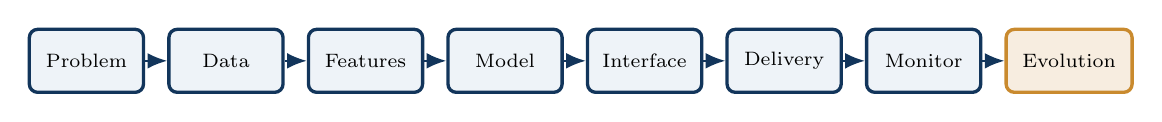
\begin{tikzpicture}[node distance=0.28cm]
  \node[flowbox, minimum width=1.45cm, minimum height=0.8cm] (problem) {\scriptsize Problem};
  \node[flowbox, minimum width=1.45cm, minimum height=0.8cm, right=of problem] (data) {\scriptsize Data};
  \node[flowbox, minimum width=1.45cm, minimum height=0.8cm, right=of data] (features) {\scriptsize Features};
  \node[flowbox, minimum width=1.45cm, minimum height=0.8cm, right=of features] (model) {\scriptsize Model};
  \node[flowbox, minimum width=1.45cm, minimum height=0.8cm, right=of model] (interface) {\scriptsize Interface};
  \node[flowbox, minimum width=1.45cm, minimum height=0.8cm, right=of interface] (delivery) {\scriptsize Delivery};
  \node[flowbox, minimum width=1.45cm, minimum height=0.8cm, right=of delivery] (monitor) {\scriptsize Monitor};
  \node[accentbox, minimum width=1.6cm, minimum height=0.8cm, right=of monitor] (evolution) {\scriptsize Evolution};
  \foreach \a/\b in {problem/data,data/features,features/model,model/interface,interface/delivery,delivery/monitor,monitor/evolution} {
    \draw[arrow] (\a) -- (\b);
  }
  \end{tikzpicture}

  \vspace{0.5em}
  \begin{block}{Today in the course}
  \textbf{Focus:} #1

  \textbf{Bridge:} #2
  \end{block}

  \begin{columns}[T]
  \column{0.48\textwidth}
  \begin{block}{Fraud case}
  {\footnotesize #3}
  \end{block}
  \column{0.48\textwidth}
  \begin{block}{Pasteurization case}
  {\footnotesize #4}
  \end{block}
  \end{columns}

  \vspace{0.3em}
  {\footnotesize \textbf{Course thread:} #5}
  \coursefooter
  \end{frame}
}

\newcommand{\classclosingframe}[4]{
  \begin{frame}{From This Class to the Next}
  \begin{block}{What stays with us}
  #1
  \end{block}

  \begin{columns}[T]
  \column{0.48\textwidth}
  \begin{block}{Project use}
  {\footnotesize #2}
  \end{block}
  \column{0.48\textwidth}
  \begin{block}{Next connection}
  {\footnotesize #3}
  \end{block}
  \end{columns}

  \vspace{0.3em}
  {\footnotesize \textbf{Course thread:} #4}
  \coursefooter
  \end{frame}
}

\tikzset{
  flowbox/.style={
    rounded corners=3pt,
    draw=courseblue,
    fill=courseice,
    very thick,
    minimum width=2.2cm,
    minimum height=0.9cm,
    align=center,
    font=\small
  },
  accentbox/.style={
    rounded corners=3pt,
    draw=coursegold,
    fill=coursegold!15,
    very thick,
    minimum width=2.2cm,
    minimum height=0.9cm,
    align=center,
    font=\small
  },
  arrow/.style={
    -{Latex[length=2.5mm,width=2mm]},
    thick,
    draw=courseblue
  }
}


\title{Class 25: Pasteurization Monitoring Challenge}
\subtitle{A two-session practice in requirements, specification, validation, and evolution}
\author{\coursename}
\date{}

\begin{document}
\frame{\titlepage \coursefooter}

\begin{frame}{The challenge in one sentence}
\begin{block}{NorthRiver Dairy needs a monitoring and alerting application}
Student teams will specify, build, validate, and evolve a Streamlit application that consumes a live pasteurization stream and helps operators notice abnormal conditions.
\end{block}
\begin{itemize}
\item This is a \textbf{requirements and development-process} exercise, not a competition to build the most elaborate dashboard.
\item The live simulator is the shared operational environment; the team product is the monitoring and alerting client.
\item Every feature must trace from a stakeholder need to a requirement, acceptance check, implementation, and test.
\end{itemize}
\coursefooter
\end{frame}

\begin{frame}{Two-session roadmap}
\centering
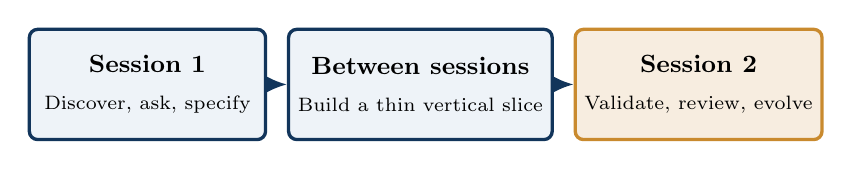
\begin{tikzpicture}[node distance=0.25cm]
\node[flowbox, minimum width=3.0cm, minimum height=1.4cm] (a) {\textbf{Session 1}\\[0.25em]\scriptsize Discover, ask, specify};
\node[flowbox, minimum width=3.0cm, minimum height=1.4cm, right=of a] (b) {\textbf{Between sessions}\\[0.25em]\scriptsize Build a thin vertical slice};
\node[accentbox, minimum width=3.0cm, minimum height=1.4cm, right=of b] (c) {\textbf{Session 2}\\[0.25em]\scriptsize Validate, review, evolve};
\draw[arrow] (a) -- (b); \draw[arrow] (b) -- (c);
\end{tikzpicture}
\vspace{0.7em}
\begin{tabularx}{\textwidth}{>{\bfseries}l X X}
& Main activity & Main evidence \\
\toprule
1 & Elicitation, analysis, SRS baseline, plan & Questions, backlog, SRS v1, process model \\
2 & Demonstration, validation, change request & Tests, traceability, SRS v2, release notes \\
\bottomrule
\end{tabularx}
\coursefooter
\end{frame}

\begin{frame}{Learning objectives}
\learninggoals{\begin{itemize}
\item Turn an incomplete stakeholder narrative into functional, non-functional, domain, and operational requirements.
\item Write a concise IEEE-style Software Requirements Specification (SRS) that is testable and traceable.
\item Use an agile, iterative process model with explicit artifacts, milestones, feedback, and change control.
\item Validate a working increment against acceptance criteria using a live external stream.
\item Explain how a requirement change affects requirements, tests, code, and release decisions.
\end{itemize}}
\coursefooter
\end{frame}

\coursecontextframe
{A dairy operator can observe raw sensor values but has no unified way to configure alerts, understand their severity, or retain a record of what happened during a batch.}
{NorthRiver Dairy requests a lightweight monitoring and alerting application. It informs people; it never controls the equipment.}
{The case brief is deliberately incomplete. Asking focused questions and recording assumptions is part of the assessed work.}
{Use the English case brief in \texttt{documents/Class25\_Pasteurization\_Monitoring\_Challenge.md}.}
{Do not begin with widgets. Begin with decisions, users, consequences, and evidence.}

\begin{frame}{The shared live simulator}
\begin{block}{Server}\url{https://four40mi-pasteurization-simulator.onrender.com}\end{block}
\begin{block}{Team stream}\url{https://four40mi-pasteurization-simulator.onrender.com/stream?team=G01}\end{block}
Replace \texttt{G01} with your assigned team identifier. The service uses Server-Sent Events (SSE): event \texttt{sensor-reading} carries JSON observations.
\begin{itemize}
\item The shared global clock gives teams equivalent observations when they connect at the same time.
\item Fields include \texttt{timestamp}, \texttt{event\_id}, \texttt{batch\_id}, \texttt{state}, \texttt{T}, \texttt{pH}, \texttt{P}, \texttt{Kappa}, \texttt{Mu}, \texttt{Tau}, \texttt{Q\_in}, \texttt{Q\_out}, and \texttt{dTdt}.
\item Schema: \url{https://four40mi-pasteurization-simulator.onrender.com/schema}
\end{itemize}
\coursefooter
\end{frame}

\begin{frame}{Product scope: make the boundary explicit}
\begin{columns}[T]
\column{0.48\textwidth}\begin{block}{In scope for the MVP}\begin{itemize}
\item Connect to and visualize live data.
\item Show connection, batch, and current state.
\item Configure selected alert rules.
\item Display severity, active alerts, and local history.
\item Acknowledge alerts and explain why they occurred.
\end{itemize}\end{block}
\column{0.48\textwidth}\begin{block}{Outside scope}\begin{itemize}
\item Sending commands to heaters, pumps, or valves.
\item Modifying the simulator or its stream contract.
\item Replacing quality procedures or a plant safety system.
\item Enterprise identity management in the first release.
\end{itemize}\end{block}
\end{columns}
\begin{alertblock}{Important}An attractive chart is not a requirement. State the user, trigger, behavior, constraint, and acceptance evidence.\end{alertblock}
\coursefooter
\end{frame}

\begin{frame}{The process model teams will apply}
\centering
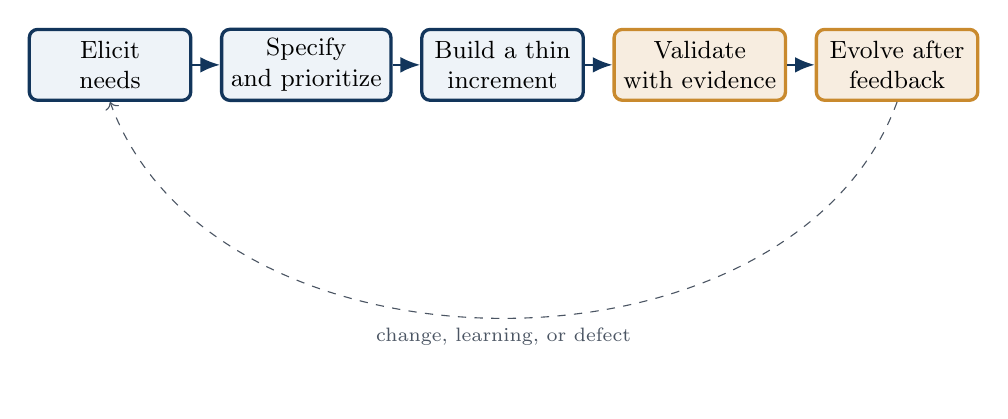
\begin{tikzpicture}[node distance=0.35cm]
\node[flowbox, minimum width=2.05cm] (elicit) {Elicit\\needs};
\node[flowbox, minimum width=2.05cm, right=of elicit] (spec) {Specify\\and prioritize};
\node[flowbox, minimum width=2.05cm, right=of spec] (build) {Build a thin\\increment};
\node[accentbox, minimum width=2.05cm, right=of build] (valid) {Validate\\with evidence};
\node[accentbox, minimum width=2.05cm, right=of valid] (evolve) {Evolve after\\feedback};
\draw[arrow] (elicit) -- (spec); \draw[arrow] (spec) -- (build); \draw[arrow] (build) -- (valid); \draw[arrow] (valid) -- (evolve);
\draw[coursegray, dashed, ->] (evolve.south) to[out=-110,in=-70] node[below, font=\scriptsize] {change, learning, or defect} (elicit.south);
\end{tikzpicture}
\vspace{0.55em}
\begin{itemize}
\item This is an \textbf{iterative-incremental agile process}: specification is sufficient to start a small, testable slice, then evolves with feedback.
\item Each team adapts this model into its own workflow: roles, board states, Definition of Ready, Definition of Done, review point, and change rule.
\end{itemize}
\coursefooter
\end{frame}

\begin{frame}{Session 1: discovery and specification}
\begin{enumerate}
\item Read the case brief; identify stakeholders, decisions supported, risks, assumptions, and open questions.
\item Conduct a short stakeholder interview with the instructor. Record answers and unanswered questions.
\item Build a prioritized product backlog with user stories and acceptance criteria.
\item Write SRS v1 and agree a minimum viable increment.
\item Define the team process and plan the first increment.
\end{enumerate}
\begin{block}{Question discipline}Ask questions that reduce uncertainty: ``Who configures this?'', ``What makes an alert critical?'', ``What evidence is required?'', ``What happens if data is missing?''\end{block}
\coursefooter
\end{frame}

\begin{frame}{SRS v1: concise, IEEE-style, and useful}
\begin{tabularx}{\textwidth}{>{\bfseries}l X}
Section & Minimum content \\
\toprule
Introduction & Purpose, scope, stakeholders, definitions, assumptions \\
Overall description & Users, operating environment, external SSE interface, constraints \\
Functional requirements & Identified \texttt{FR-xx} statements written with ``shall'' \\
Non-functional requirements & Measurable usability, performance, reliability, maintainability, and security expectations \\
Domain and business rules & Alert concepts, severity, process-state rules, traceability expectations \\
Operational requirements & Start-up, configuration, disconnection, recovery, support, known limitations \\
Validation and traceability & Acceptance criteria, test idea, priority, dependencies \\
\bottomrule
\end{tabularx}
\vspace{0.3em}\begin{block}{Quality check}One requirement should express one observable obligation. Avoid ``fast'', ``easy'', ``robust'', or ``real time'' unless the statement says how it will be checked.\end{block}
\coursefooter
\end{frame}

\begin{frame}{From a story to evidence}
\begin{block}{User story}As a plant operator, I want to see a clearly classified active alert so that I can decide whether the current batch needs attention.\end{block}
\begin{block}{Possible system requirement}When an evaluated reading violates a configured rule, the system \textbf{shall} create an alert containing the batch identifier, sensor, configured rule, observed value, timestamp, process state, and severity.\end{block}
\begin{block}{Possible acceptance criterion}Given a configured temperature rule and a violating reading, when the configured persistence condition is met, then the dashboard displays one active alert with all required fields and stores it in session history.\end{block}
\coursefooter
\end{frame}

\begin{frame}{Session 2: validation and evolution}
\begin{enumerate}
\item Demonstrate the thin increment against agreed acceptance criteria.
\item Use the live stream to gather evidence: normal behavior, threshold crossing, and disconnection behavior.
\item Review the traceability matrix and identify defects, gaps, and assumptions.
\item Receive the change request from Quality Management.
\item Analyze impact, reprioritize the backlog, update SRS v1 to v2, and implement or plan the evolution.
\end{enumerate}
\begin{block}{Change request}During \texttt{Hold}, temperature violations become critical only after a configurable number of consecutive readings. The recorded alert must include the process state in which it was raised.\end{block}
\coursefooter
\end{frame}

\begin{frame}{Milestones and artifacts}
\begin{tabularx}{\textwidth}{>{\bfseries}l X X}
Milestone & Decision gate & Required artifact \\
\toprule
M1 Discovery & Do we understand the problem enough to proceed? & Stakeholder map, question log, glossary, assumptions \\
M2 Baseline & Is the first increment small and testable? & Backlog, SRS v1, acceptance criteria, process model \\
M3 MVP & Does the vertical slice work? & Streamlit application, code, demonstration \\
M4 Validation & What evidence supports the claims? & Test record, defects, traceability matrix \\
M5 Evolution & What changes and why? & Change analysis, SRS v2, backlog update, release notes \\
\bottomrule
\end{tabularx}
\coursefooter
\end{frame}

\begin{frame}{Operational requirements are part of the product}
\begin{block}{Operational guide: minimum contents}\begin{itemize}
\item How to start the Streamlit application and select a team stream.
\item How to configure, save, reset, and interpret alert rules.
\item Meaning of severities, acknowledgement, active versus historic alert.
\item Behavior on malformed data, missing values, or stream disconnection.
\item Recovery steps, known limitations, and explicit statement that the application does not control equipment.
\end{itemize}\end{block}
\begin{alertblock}{Operational thinking}If the app is correct only when the stream is perfect, the requirement is incomplete.\end{alertblock}
\coursefooter
\end{frame}

\begin{frame}{Instructor as the stakeholder panel}
\begin{itemize}
\item The instructor plays Operations Manager, Quality Manager, and Senior Plant Operator.
\item Teams ask questions; the instructor gives the same canonical answer to every team and adds it to a shared answer log.
\item When a business decision is genuinely open, teams propose alternatives, record an assumption, and justify their choice.
\item Do not silently invent a requirement. Mark the source: stakeholder answer, observed stream behavior, team assumption, or technical constraint.
\end{itemize}
\begin{block}{Facilitation guide}The case brief includes a private instructor section with recommended answers, disclosure timing, and discussion prompts.\end{block}
\coursefooter
\end{frame}

\begin{frame}{Assessment: evidence over interface polish}
\begin{tabularx}{\textwidth}{>{\bfseries}l X}
Criterion & What good evidence looks like \\
\toprule
Requirements quality & Clear scope; distinguishable FR/NFR/domain/operational requirements; testable wording \\
Elicitation and reasoning & Focused questions, explicit assumptions, trade-offs, stakeholder rationale \\
Process discipline & Credible iterative workflow, prioritized work, Definition of Done, change handling \\
Traceability and validation & Requirement $\rightarrow$ acceptance criterion $\rightarrow$ implementation $\rightarrow$ test result \\
Working increment & Reliable connection, understandable status, configured alert behavior, useful evidence \\
Evolution & Impact analysis and coherent SRS/backlog/test changes after the new rule \\
\bottomrule
\end{tabularx}
\coursefooter
\end{frame}

\classclosingframe
{\begin{itemize}\item The simulator is a source of evidence, not the specification.\item Agile work is disciplined learning: small increments, explicit decisions, and feedback that changes the plan.\item A requirement is complete only when somebody can decide whether it has been met.\end{itemize}}
{Begin with the case brief, form a team, and prepare questions before deciding what to build.}
{Class 34 develops the practical agile toolkit: boards, refinement, estimation, reviews, quality practices, and common failure modes.}
{The strongest prototype is the one whose behavior can be explained and defended from stakeholder need to validation evidence.}
\end{document}
